% Chapter 3: Release 1 (Cryptographic Foundations and Access Control)

\chapter{Release 1}
\label{ch:chapter3}

\section{Introduction}
This chapter details the conceptualization, design, and implementation of Release 1, which establishes the core infrastructural foundation of the platform. This release is divided into two structural sprints: Sprint 1 focuses on secure user authentication and profile management, while Sprint 2 is dedicated to server provisioning, channel architecture, and role-based access control. For each sprint, we outline the product backlog, analyze the dynamic and static system designs using UML modeling, and conclude by demonstrating the implemented interfaces that validate the functional requirements.

\section{Sprint 1}
This section presents the conceptual study and implementation of Sprint 1 of Release 1. We will focus primarily on the "Authentication" and profile management features, which ensure secure access to the platform.

\subsection{Sprint 1 Overview}
The primary objective of Sprint 1 is to implement secure credentials handling and authenticated session management. The user stories allocated to this sprint are described in Table~\ref{tab:sprint1_backlog}.

    
\renewcommand{\arraystretch}{1.5}
\begin{longtable}{| p{1.4cm} | p{10cm} | p{1.8cm} | p{1.5cm} |}
    \hline
    \rowcolor{lightgray}
    \textbf{ID} & \textbf{User Story \& Acceptance Criteria} & \textbf{Priority} & \textbf{Points} \\
    \hline
    \endfirsthead
    \hline
    \rowcolor{lightgray}
    \textbf{ID} & \textbf{User Story \& Acceptance Criteria} & \textbf{Priority} & \textbf{Points} \\
    \hline
    \endhead
    \hline
    \endfoot
    \hline
    \endlastfoot
\renewcommand{\arraystretch}{1.0} % Reset spacing for the rest of the document

    S1-01 & \textbf{As a} new user, \textbf{I want to} register an account with my email and a password, \textbf{so that} I can access the platform.
    \newline \textit{Acceptance Criteria}:
    \newline \textbullet\ Registration succeeds with valid data.
    \newline \textbullet\ Duplicate email is rejected.
    \newline \textbullet\ Password is stored securely (not in plain text). & P0 & 3 \\
    \hline
    S1-02 & \textbf{As a} registered user, \textbf{I want to} log in with my email and password, \textbf{so that} I can access my account and servers.
    \newline \textit{Acceptance Criteria}:
    \newline \textbullet\ Valid credentials return an access token.
    \newline \textbullet\ Wrong credentials are rejected with an error message.
    \newline \textbullet\ I stay logged in until I choose to log out. & P0 & 3 \\
    \hline
    S1-03 & \textbf{As a} logged-in user, \textbf{I want to} log out of my account, \textbf{so that} my session ends and no one else can use my account.
    \newline \textit{Acceptance Criteria}:
    \newline \textbullet\ Logging out clears my session.
    \newline \textbullet\ I am redirected to the text interface.
    \textbullet\ Protected pages are no longer accessible. & P1 & 1 \\
    \hline
    S1-04 & \textbf{As a} logged-in user, \textbf{I want to} view and edit my display name, \textbf{so that} other users see the name I choose.
    \newline \textit{Acceptance Criteria}:
    \newline \textbullet\ I can see my current display name.
    \newline \textbullet\ I can update it and the change is saved.
    \textbullet\ Other users see the updated name. & P1 & 2 \\
    \hline
    \caption{\textbf{Sprint 1 Backlog - Authentication \& Profile.}}
    \label{tab:sprint1_backlog} \\
\end{longtable}

\subsection{Analysis and design of sprint 1}
In this stage of Sprint 1, we will focus on the authentication implementation by carrying out a thorough analysis and outlining its conceptual design.

\subsubsection{Use case diagram}
A use case diagram illustrates the interactions between users (actors) and the system, showing the different ways in which users can engage with the system.

\begin{figure}[H]
    \centering
    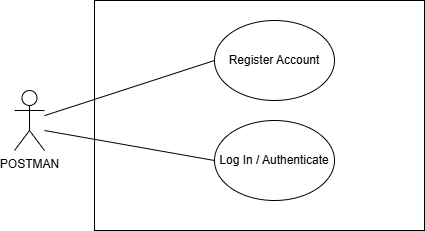
\includegraphics[width=0.8\textwidth]{use_case_sprint1_plantuml.png}
    \caption{Use Case Diagram for Sprint 1 - Authentication \& Profile.}
    \label{fig:use_case_sprint1}
\end{figure}

\subsubsection{Activity Diagram}
An activity diagram illustrates the dynamic flow of control from one activity to another, detailing the step-by-step processes of a specific use case. The figure below presents the activity diagram for the authentication process, covering both successful login and potential failure paths (e.g., invalid credentials).

\begin{figure}[H]
    \centering
    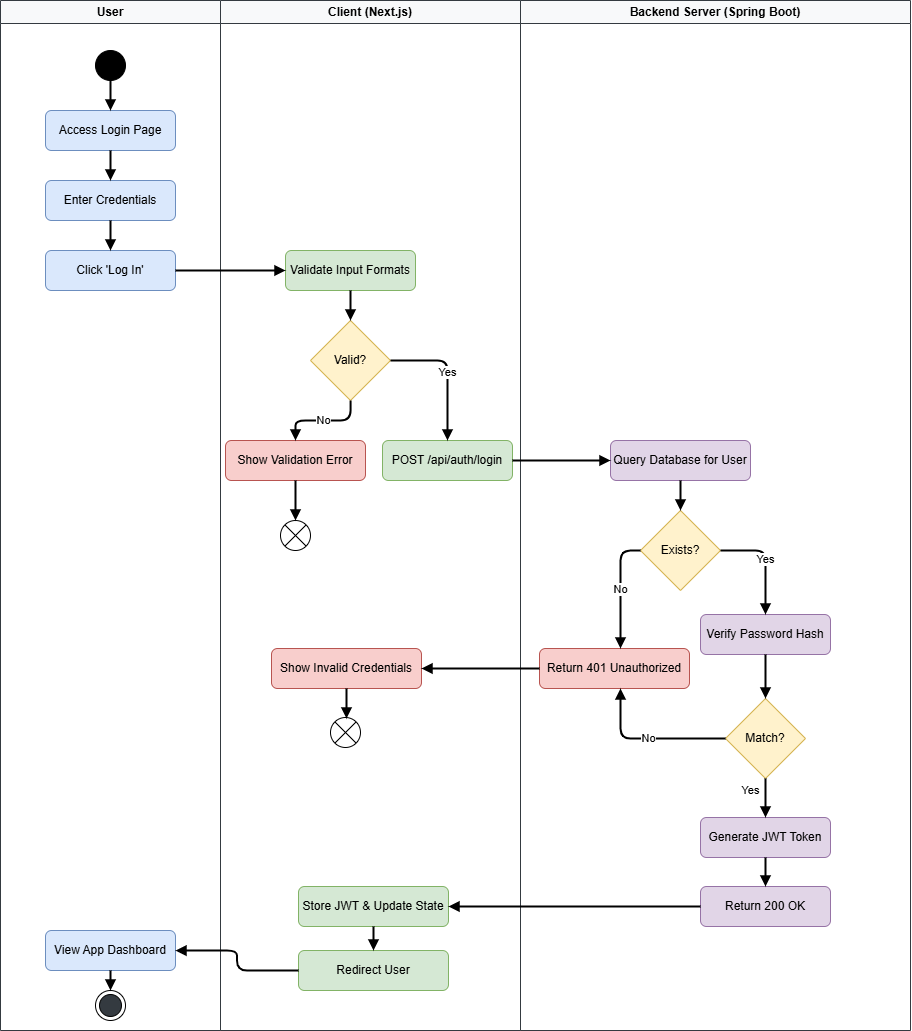
\includegraphics[width=0.9\textwidth]{auth_activity_diag.png}
    \caption{Activity Diagram for User Authentication (Success and Failure Paths).}
    \label{fig:auth_activity_sprint1}
\end{figure}

\subsubsection{Class Diagram}
The class diagram below details the static structure of the authentication entities, including the User, JWT Token, and cryptographic vault components.

\begin{figure}[H]
    \centering
    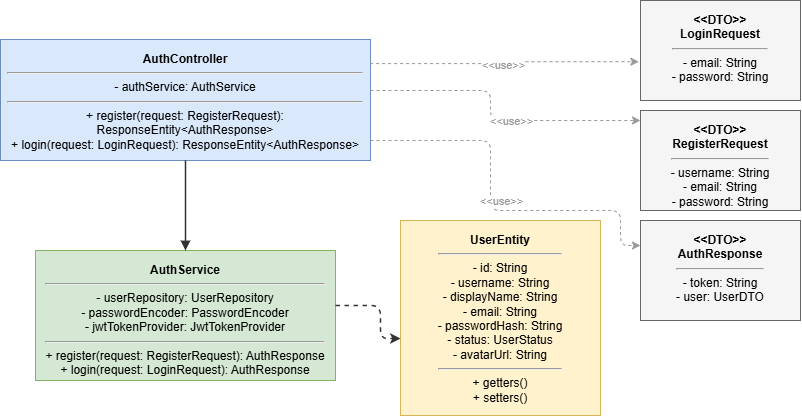
\includegraphics[width=0.8\textwidth]{auth_class_sprint1.png}
    \caption{Class Diagram for JWT Authentication.}
    \label{fig:sprint1_class_auth}
\end{figure}

\subsubsection{Design Sequence Diagram}
The sequence diagram below illustrates the operation flow and transition among the various layers of the application during the user login process:

\begin{figure}[H]
    \centering
    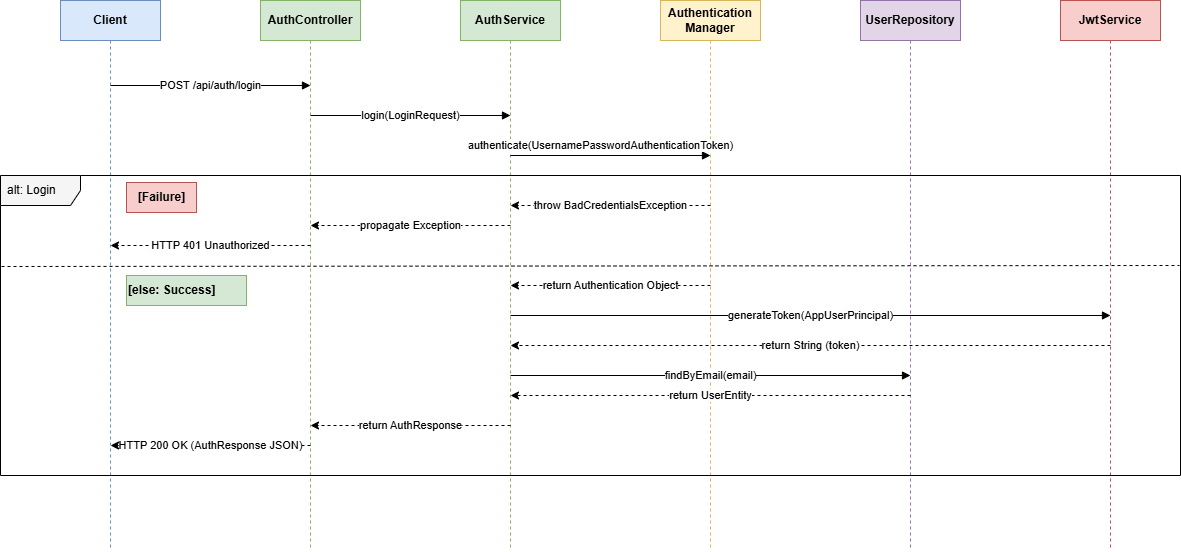
\includegraphics[width=0.9\textwidth]{seq_diag_sprint1.png}
    \caption{Secure JWT Token Exchange Sequence Diagram.}
    \label{fig:sprint1_seq_auth}
\end{figure}

\subsection{Review}
To validate the authentication process, we executed API tests using Postman. The figures below illustrate the server responses for both successful and failed login attempts.

\begin{figure}[H]
    \centering
    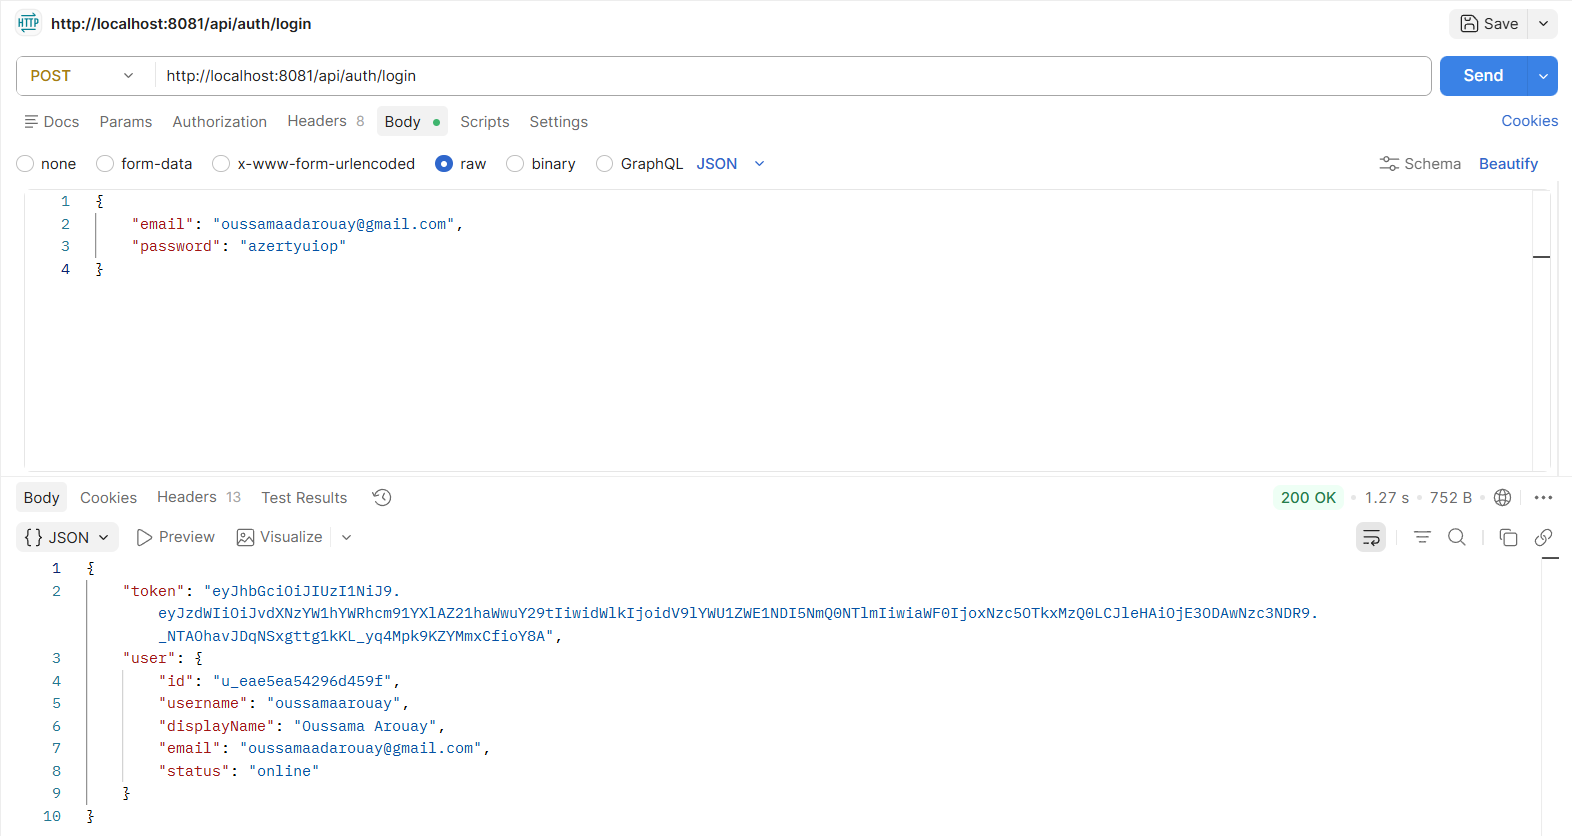
\includegraphics[width=0.8\textwidth]{login_test_success.png}
    \caption{Postman: Successful Login.}
    \label{fig:postman_login_success}
\end{figure}

\begin{figure}[H]
    \centering
    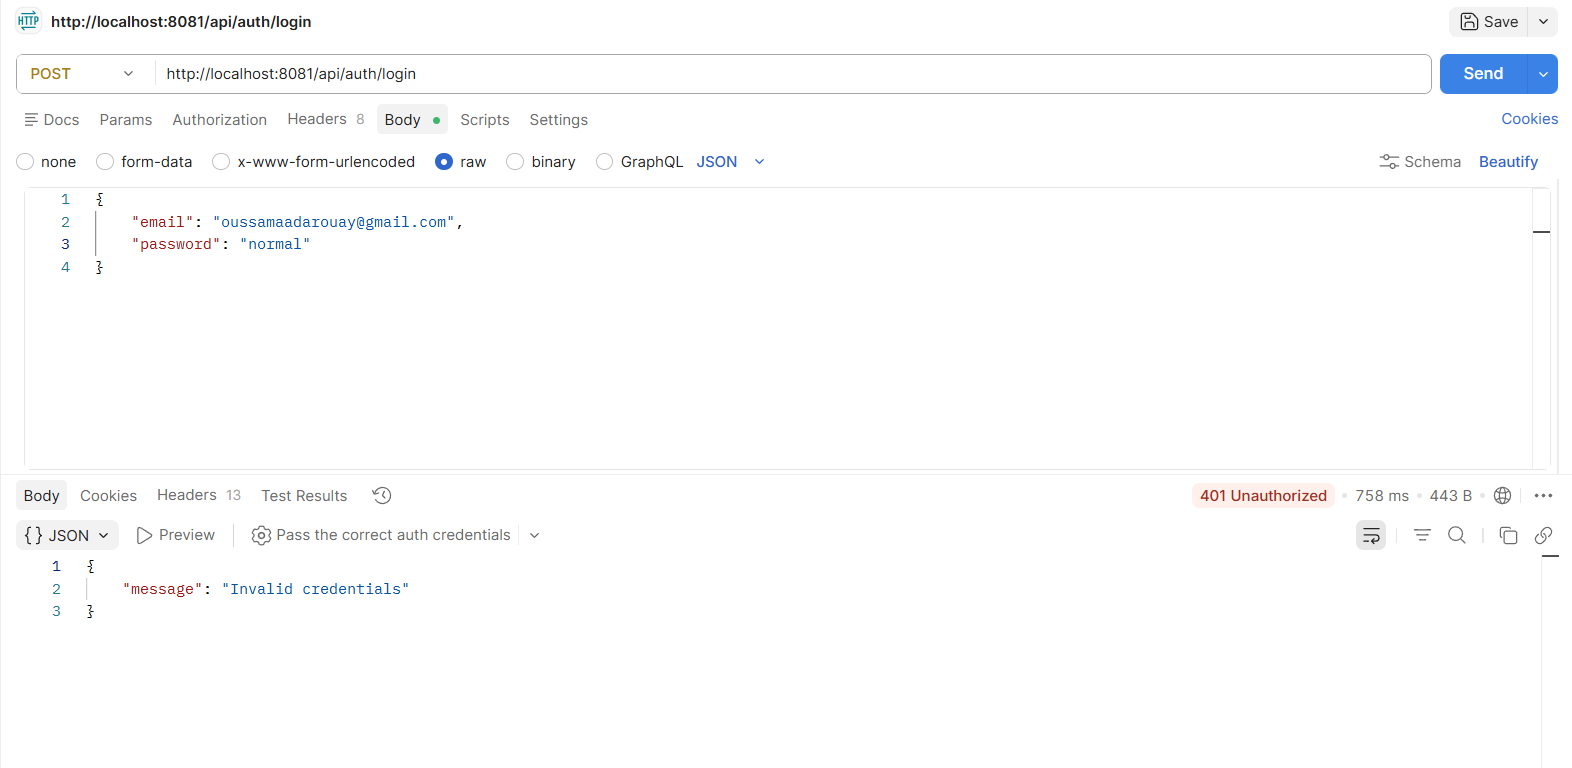
\includegraphics[width=0.8\textwidth]{login_test_failure.png}
    \caption{Postman: Failed Login Attempt (Invalid Credentials).}
    \label{fig:postman_login_failure}
\end{figure}

\section{Sprint 2: Server Management and Data Isolation}
This section presents the conceptual study and implementation of Sprint 2 of Release 1. We will focus primarily on server provisioning, channel architecture, and role-based permissions, which establish secure community workspaces within the platform.

\subsection{Sprint 2 Overview}
This sprint focuses on secure server creation, invite links, and granular channel configurations with role-based access control.

\subsection{Sprint 2 Backlog}
The primary objective of Sprint 2 is to deploy secure server configurations and member access controls. The user stories allocated to this sprint are described in Table~\ref{tab:sprint2_backlog}.

    
\renewcommand{\arraystretch}{1.5}
\begin{longtable}{| p{1.4cm} | p{10cm} | p{2.0cm} | p{1.5cm} |}
    \hline
    \rowcolor{lightgray}
    \textbf{ID} & \textbf{User Story \& Acceptance Criteria} & \textbf{Priority} & \textbf{Points} \\
    \hline
    \endfirsthead
    \hline
    \rowcolor{lightgray}
    \textbf{ID} & \textbf{User Story \& Acceptance Criteria} & \textbf{Priority} & \textbf{Points} \\
    \hline
    \endhead
    \hline
    \endfoot
    \hline
    \endlastfoot
\renewcommand{\arraystretch}{1.0} % Reset spacing for the rest of the document

    S2-01 & \textbf{As a} user, \textbf{I want to} create a new server, \textbf{so that} I have a private space to invite my friends.
    \newline \textit{Acceptance Criteria}:
    \newline \textbullet\ The server is created with the name I chose.
    \newline \textbullet\ I am automatically its owner.
    \newline \textbullet\ A default text channel is created inside it. & P0 & 3 \\
    \hline
    S2-02 & \textbf{As a} server owner, \textbf{I want to} generate an invite link for my server, \textbf{so that} I can share it with friends so they can join.
    \newline \textit{Acceptance Criteria}:
    \newline \textbullet\ A unique invite link is generated.
    \newline \textbullet\ Anyone with the link can join the server.
    \newline \textbullet\ The link expires after 24 hours. & P0 & 3 \\
    \hline
    S2-03 & \textbf{As a} user, \textbf{I want to} join a server using an invite link, \textbf{so that} I can participate in that community.
    \newline \textit{Acceptance Criteria}:
    \newline \textbullet\ Clicking a valid link adds me to the server.
    \newline \textbullet\ An expired or invalid link shows an error.
    \newline \textbullet\ I can see the server's channels after joining. & P0 & 2 \\
    \hline
    S2-04 & \textbf{As a} server owner, \textbf{I want to} create text and voice channels inside my server, \textbf{so that} I can organize conversations by topic.
    \newline \textit{Acceptance Criteria}:
    \newline \textbullet\ I can create a channel with a name and a type (text or voice).
    \newline \textbullet\ The channel appears in the server sidebar.
    \newline \textbullet\ Only the owner or admins can create channels. & P1 & 3 \\
    \hline
    S2-05 & \textbf{As a} server owner, \textbf{I want to} create roles and assign them to members, \textbf{so that} I can delegate responsibilities and control who can do what.
    \newline \textit{Acceptance Criteria}:
    \newline \textbullet\ I can create a role with a name and a set of permissions.
    \newline \textbullet\ I can assign a role to a member.
    \textbullet\ A member's permissions update immediately after assignment. & P1 & 5 \\
    \hline
    S2-06 & \textbf{As a} server member, \textbf{I want to} leave a server I no longer want to be part of, \textbf{so that} I am not in servers that are no longer relevant to me.
    \newline \textit{Acceptance Criteria}:
    \newline \textbullet\ Leaving removes me from the member list.
    \newline\textbullet\ I can no longer see the server's channels.
    \textbullet\ The server owner cannot leave without transferring ownership. & P2 & 2 \\
    \hline
    \caption{\textbf{Sprint 2 Backlog - Servers, Channels \& Permissions.}}
    \label{tab:sprint2_backlog} \\
\end{longtable}
\normalsize

\subsection{Analysis and design of sprint 2}
In this stage of Sprint 2, we focus on the architecture of server management and access control by outlining its conceptual design.

\subsubsection{Use case diagram}
The use case diagram below illustrates the interactions between authenticated users, server members, and server owners regarding the features implemented in this sprint.

\begin{figure}[H]
    \centering
    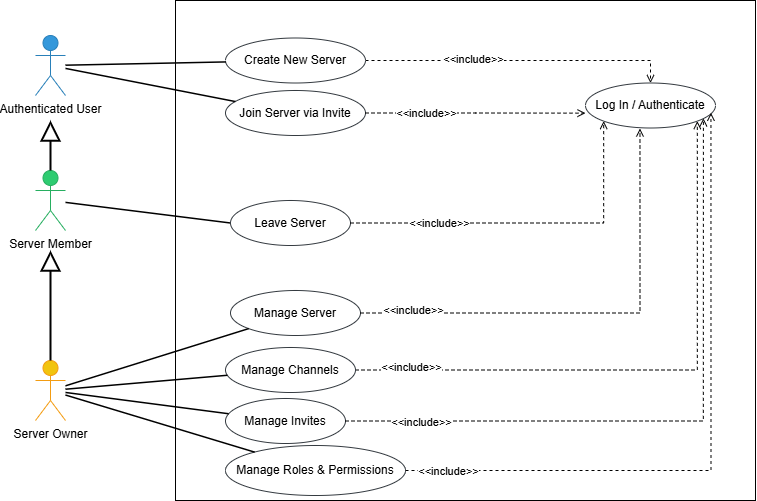
\includegraphics[width=0.8\textwidth]{UseCase_sprint2.png}
    \caption{Use Case Diagram for Sprint 2 - Server Management.}
    \label{fig:use_case_sprint2}
\end{figure}

\subsubsection{Textual Description}
At this stage, we will detail the textual descriptions of the use cases for Sprint 2 (Create a new Server/Guild and Join a Server via Invite Link) (Tables~\ref{tab:usecase_create_server} and~\ref{tab:usecase_join_server}).

\renewcommand{\arraystretch}{1.15}
\begin{table}[H]
    \centering
    \begin{tabular}{| p{3.5cm} | p{10.5cm} |}
        \hline
        \textbf{Use Case} & Create a new Server/Guild \\
        \hline
        \textbf{Actor} & Authenticated User \\
        \hline
        \textbf{Pre-condition} & The actor must be logged into the platform with a valid session. \\
        \hline
        \textbf{Main Scenario} & 
        \vspace{-0.3cm}
        \begin{minipage}[t]{10.5cm}
            \begin{enumerate}
                \item The actor clicks on the "+" sign in the sidebar.
                \item The system prompts the actor to enter a server name.
                \item The actor submits the creation form.
                \item The system registers the new server in the database and assigns the actor as the "Owner".
                \item The system automatically generates a default "general" text channel.
            \end{enumerate}
            \vspace{0.1cm}
        \end{minipage} \\
        \hline
        \textbf{Post-condition} & A new server is created, and the user is granted absolute Owner privileges over it. \\
        \hline
    \end{tabular}
    \vspace{0.2cm}
    \caption{Textual description of "Create a new Server/Guild"}
    \label{tab:usecase_create_server}
\end{table}


\renewcommand{\arraystretch}{1.15}
\begin{table}[H]
    \centering
    \begin{tabular}{| p{3.5cm} | p{10.5cm} |}
        \hline
        \textbf{Use Case} & Join a Server via Invite Link \\
        \hline
        \textbf{Actor} & Authenticated User \\
        \hline
        \textbf{Pre-condition} & The actor is logged in, possesses a valid invite link, and is not already a member of the server. \\
        \hline
        \textbf{Main Scenario} & 
        \vspace{-0.5cm}
        \begin{minipage}[t]{10.5cm}
            \begin{enumerate}
                \item The actor clicks on a server invite link.
                \item The system validates the invite link (checks if it exists and has not expired).
                \item The system verifies that the actor is not already a member of the server.
                \item The system adds the actor to the server's member list.
                \item The system assigns the actor default roles for that server.
            \end{enumerate}
            \vspace{-0.2cm}
        \end{minipage} \\
        \hline
        \textbf{Post-condition} & The actor becomes a member of the server and gains access to its default channels. \\
        \hline
    \end{tabular}
    \vspace{0.2cm}
    \caption{Textual description of "Join Server via Invite"}
    \label{tab:usecase_join_server}
\end{table}
\renewcommand{\arraystretch}{1.0}


\subsubsection{Class Diagram}
The class diagram below illustrates the relationships between Servers, Channels, Roles, and Permissions, highlighting how cryptographic keys are associated with server entities.

\begin{figure}[H]
    \centering
    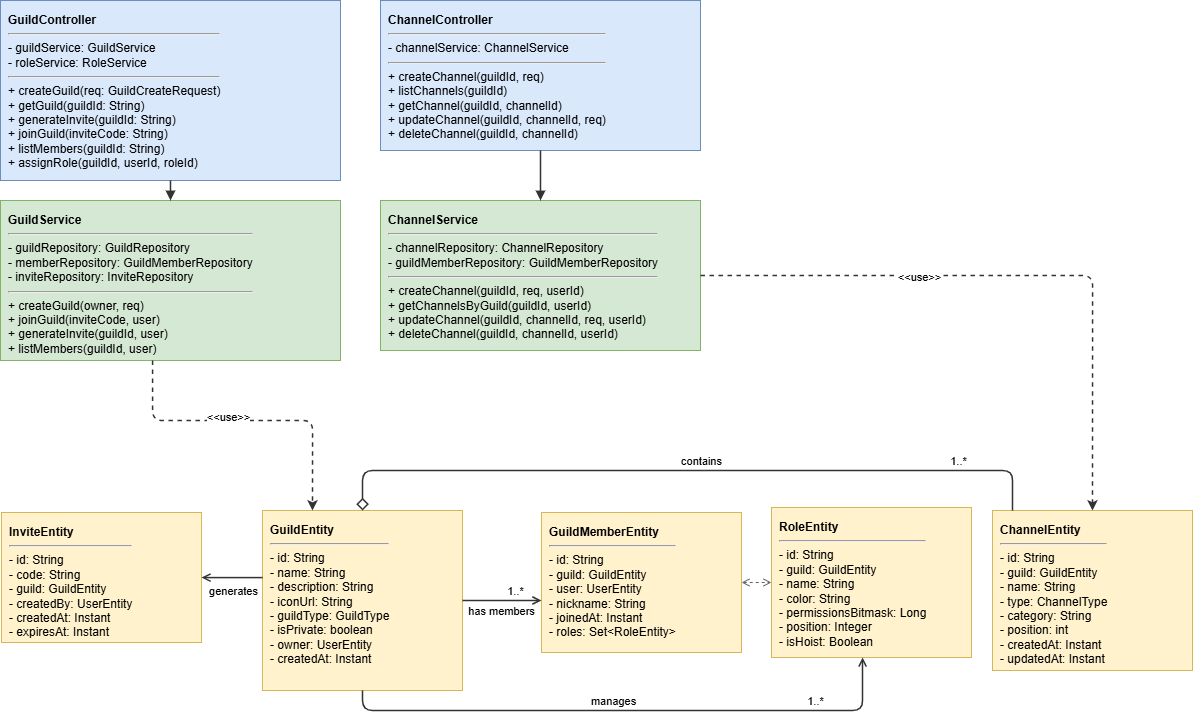
\includegraphics[width=0.8\textheight, angle=90]{class_diag_sprint2.png}
    \caption{Class Diagram for Sprint 2.}
    \label{fig:sprint2_class_perms}
\end{figure}
\subsection{Sprint 2 Review}
To validate the backend logic and operations developed during Sprint 2, we executed API tests using Postman. The figures below illustrate the successful execution of server creation, joining a server via an invite link, and creating a text channel.

\begin{figure}[H]
    \centering
    \includegraphics[width=0.8\textwidth]{{guild_creation.png}}
    \caption{Postman: Server Creation Process.}
    \label{fig:sprint2_guild_create}
\end{figure}

\begin{figure}[H]
    \centering
    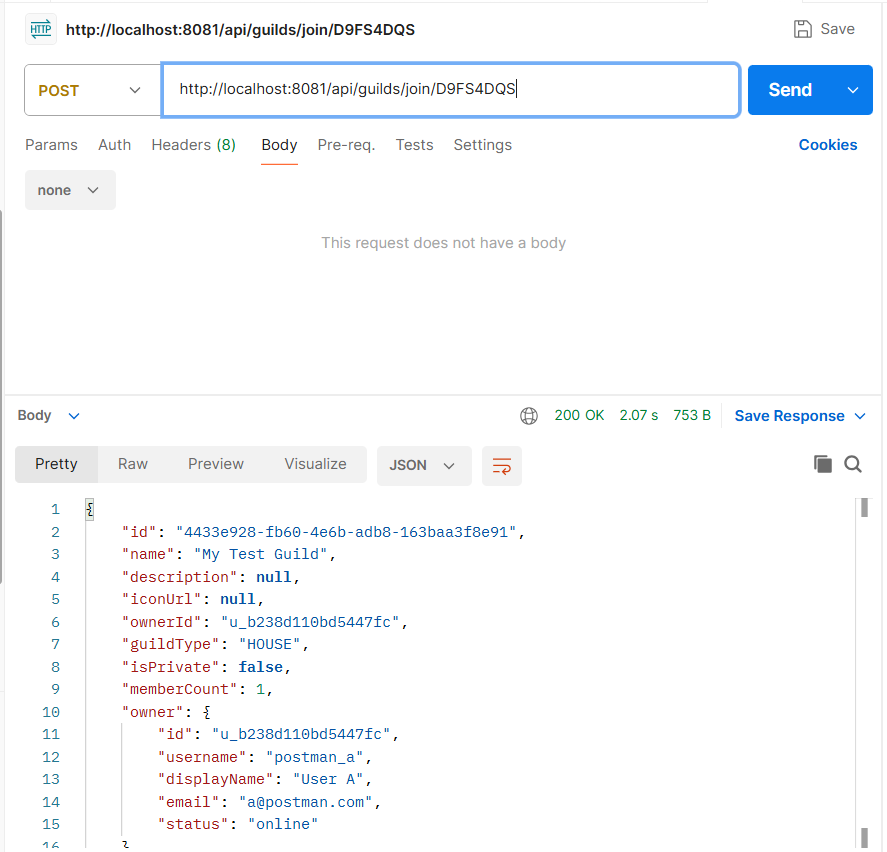
\includegraphics[width=0.8\textwidth]{guildjoin.png}
    \caption{Postman: Joining a Server via Invite.}
    \label{fig:sprint2_guild_join}
\end{figure}

\begin{figure}[H]
    \centering
    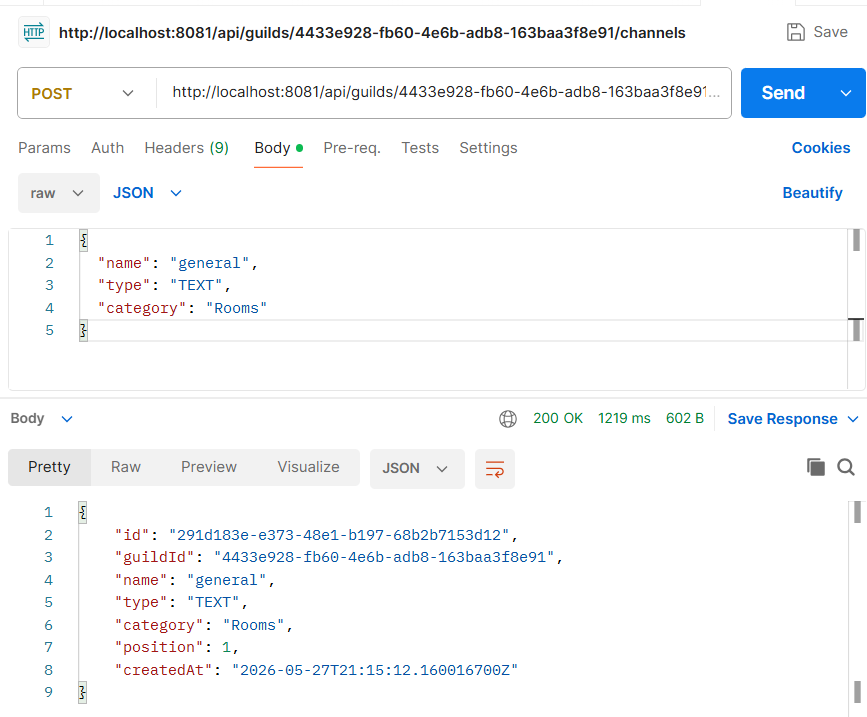
\includegraphics[width=0.8\textwidth]{textchannel creation.png}
    \caption{Postman: Creating a Text Channel.}
    \label{fig:sprint2_channel_create}
\end{figure}


\section{Conceptual Design of Release 1}

\subsection{Data Modeling}
In this section, we present the entities and tables that make up the structural foundation of our platform for this release. The data model covers user authentication, server provisioning, and role-based access control. Table~\ref{tab:data_dictionary_r1} presents the data dictionary.

\renewcommand{\arraystretch}{1.5}
\begin{longtable}{| p{4cm} | p{3.5cm} | p{7cm} |}
    \hline
    \rowcolor{lightgray}
    \textbf{Entity} & \textbf{Attribute} & \textbf{Description} \\
    \hline
    \endfirsthead
    \hline
    \rowcolor{lightgray}
    \textbf{Entity} & \textbf{Attribute} & \textbf{Description} \\
    \hline
    \endhead
    \hline
    \endfoot
    \hline
    \caption{Dictionnaire de données de la release 1.}
    \label{tab:data_dictionary_r1}
    \endlastfoot

    User (Utilisateur) & id & Unique identifier for the user. \\
    \cline{2-3}
         & email & User's email address. \\
    \cline{2-3}
         & username & User's chosen display name. \\
    \cline{2-3}
         & passwordHash & Hashed password for authentication. \\
    \cline{2-3}
         & status & Current presence status (e.g., Online, Offline). \\
    \cline{2-3}
         & dateCreated & Account creation date. \\
    \hline
    Server (Serveur) & id & Unique identifier for the server. \\
    \cline{2-3}
         & name & Name of the server. \\
    \cline{2-3}
         & ownerId & Identifier of the user who owns the server. \\
    \cline{2-3}
         & iconUrl & URL to the server's icon image. \\
    \cline{2-3}
         & dateCreated & Creation date of the server. \\
    \hline
    Channel (Canal) & id & Unique identifier for the channel. \\
    \cline{2-3}
         & serverId & Identifier of the parent server. \\
    \cline{2-3}
         & name & Name of the channel (e.g., "general"). \\
    \cline{2-3}
         & type & Type of the channel (text or voice). \\
    \cline{2-3}
         & dateCreated & Creation date of the channel. \\
    \hline
    Role (Rôle) & id & Unique identifier for the role. \\
    \cline{2-3}
         & serverId & Identifier of the server the role belongs to. \\
    \cline{2-3}
         & name & Name of the role (e.g., "Admin", "Member"). \\
    \cline{2-3}
         & permissions & Access control permissions string or bitfield. \\
    \hline
    ServerMember (Membre) & userId & Identifier of the user. \\
    \cline{2-3}
         & serverId & Identifier of the server. \\
    \cline{2-3}
         & roleId & Identifier of the assigned role. \\
    \cline{2-3}
         & joinedAt & Date the user joined the server. \\
    \hline
\end{longtable}
\renewcommand{\arraystretch}{1.0}

\begin{figure}[H]
    \centering
    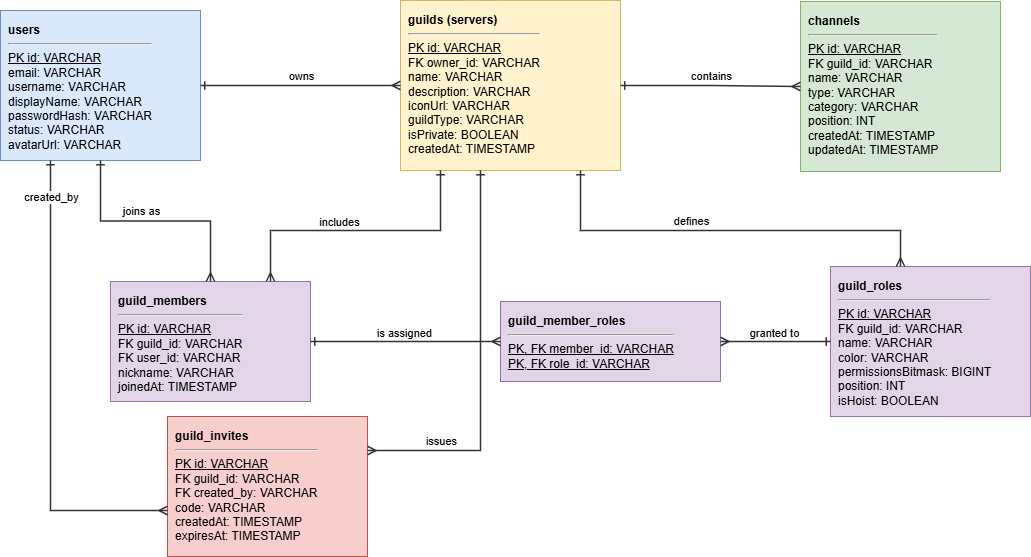
\includegraphics[width=1.1\textwidth]{release1_modele_logique_donne.png}
    \caption{Logical Data Model (MLD) for Release 1.}
    \label{fig:r1_mld}
\end{figure}

\subsubsection{Design Sequence Diagram}
We illustrate here the operation flow and transition among the various layers of an application through design sequence diagrams in this section.



\subsection{Graphical Design}
Graphical design, otherwise referred to as visual design, is an important part of visual product creation including websites, mobile apps, user interfaces, posters, logos, and ads.
In this section, we show mockup examples of our application to meet user requirements and improve user experience on a particular page.

The following figures showcase the visual design of the platform's key interfaces developed during Release 1.

\begin{figure}[H]
    \centering
    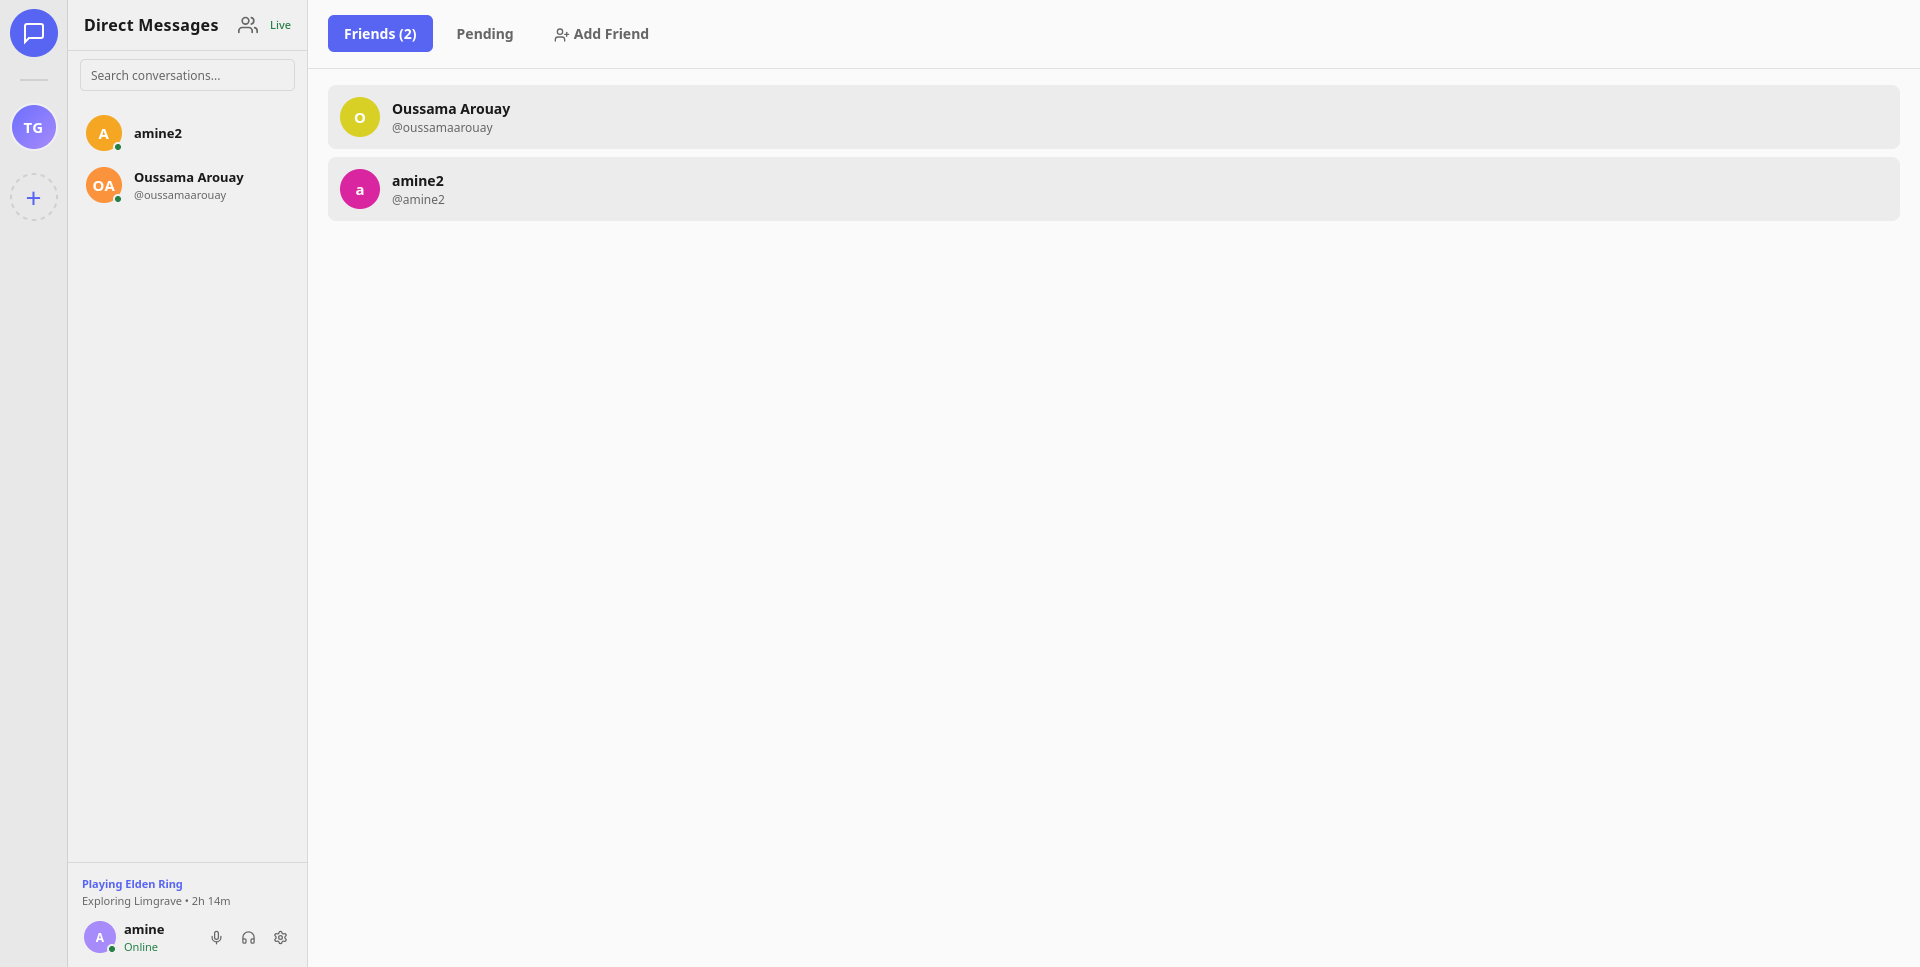
\includegraphics[width=0.85\textwidth]{landing_page_light.png}
    \caption{Mockup: Landing Page Design.}
    \label{fig:ui_landing_page}
\end{figure}

\begin{figure}[H]
    \centering
    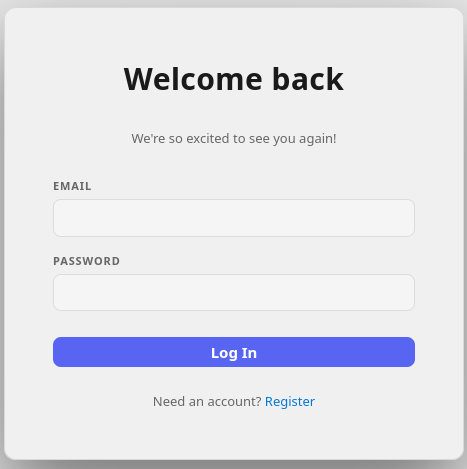
\includegraphics[width=0.5\textwidth]{login.png}
    \caption{Mockup: Login Interface.}
    \label{fig:ui_login}
\end{figure}

\begin{figure}[H]
    \centering
    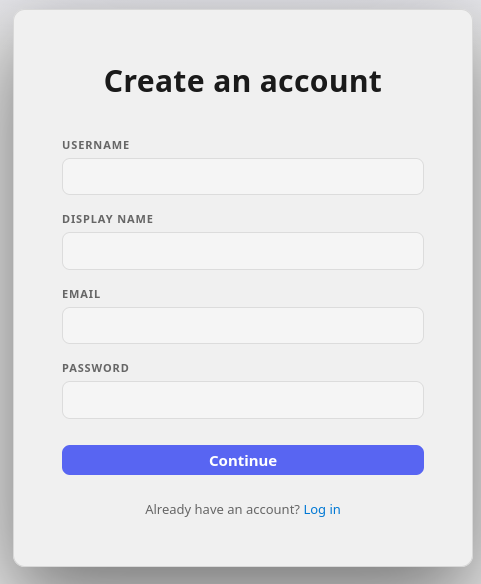
\includegraphics[width=0.5\textwidth]{singup.png}
    \caption{Mockup: Registration Interface.}
    \label{fig:ui_signup}
\end{figure}

\begin{figure}[H]
    \centering
    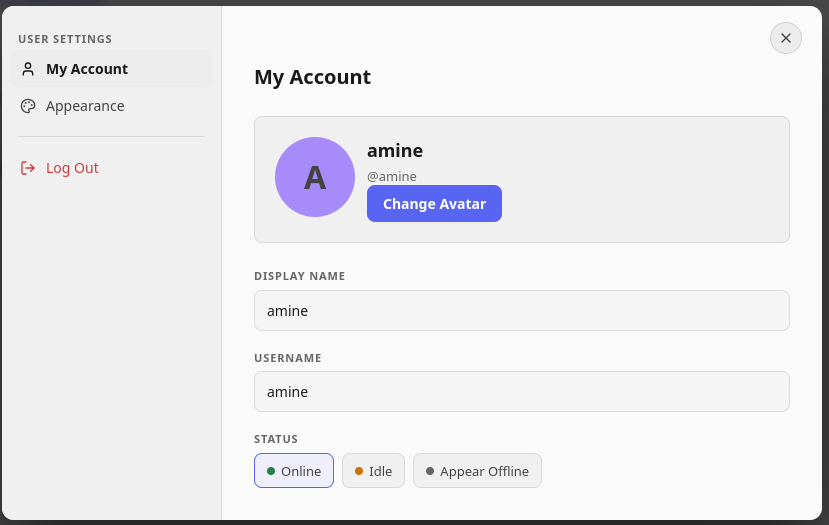
\includegraphics[width=0.5\textwidth]{user_settings.png}
    \caption{Mockup: User Settings and Profile Management.}
    \label{fig:ui_user_settings}
\end{figure}

\begin{figure}[H]
    \centering
    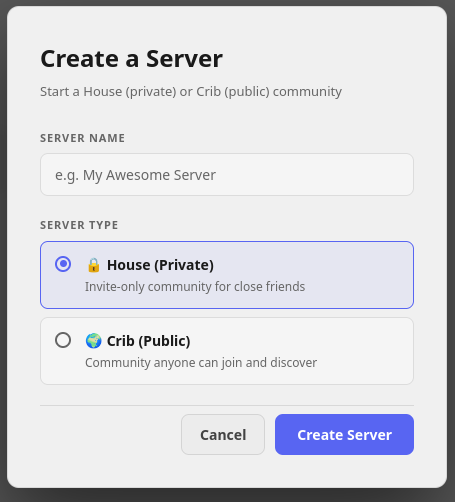
\includegraphics[width=0.4\textwidth]{create_guild.png}
    \caption{Mockup: Server Creation Interface.}
    \label{fig:ui_create_guild}
\end{figure}

\begin{figure}[H]
    \centering
    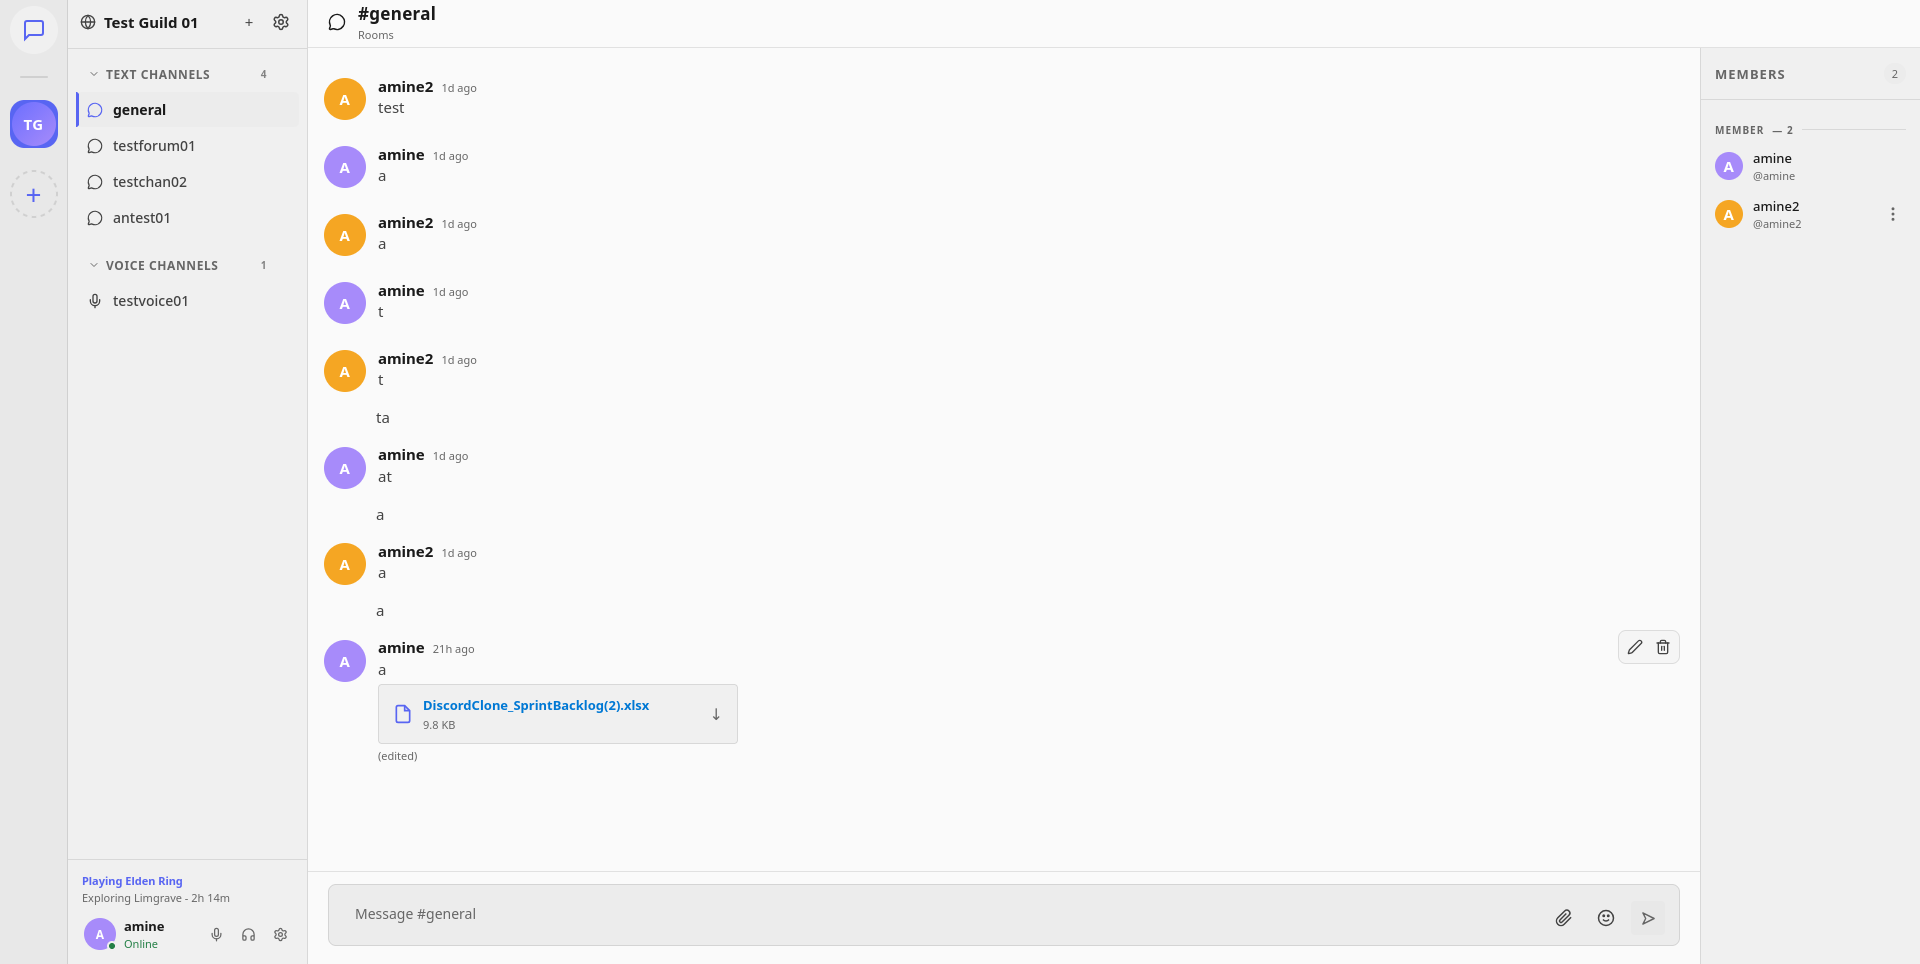
\includegraphics[width=0.85\textwidth]{main_guild_view.png}
    \caption{Mockup: Main Server View and Channel Navigation.}
    \label{fig:ui_main_guild_view}
\end{figure}

\begin{figure}[H]
    \centering
    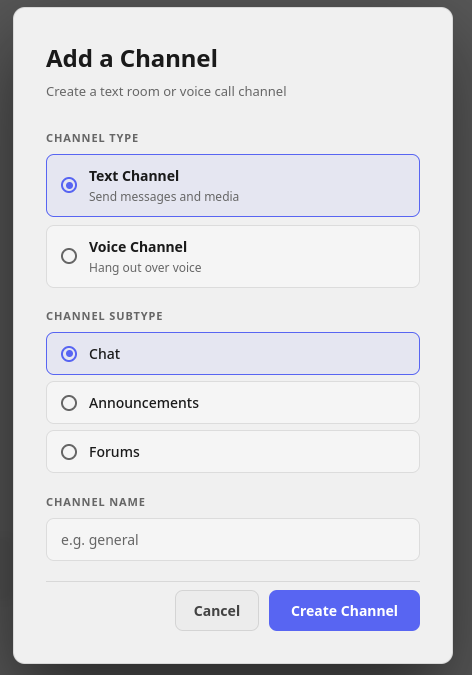
\includegraphics[width=0.5\textwidth]{add_text_channel.png}
    \caption{Mockup: Creating a Text Channel.}
    \label{fig:ui_add_text_channel}
\end{figure}

\begin{figure}[H]
    \centering
    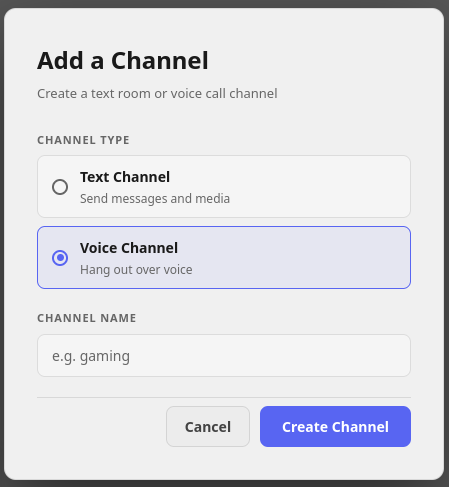
\includegraphics[width=0.5\textwidth]{add_voice_channel.png}
    \caption{Mockup: Creating a Voice Channel.}
    \label{fig:ui_add_voice_channel}
\end{figure}

\begin{figure}[H]
    \centering
    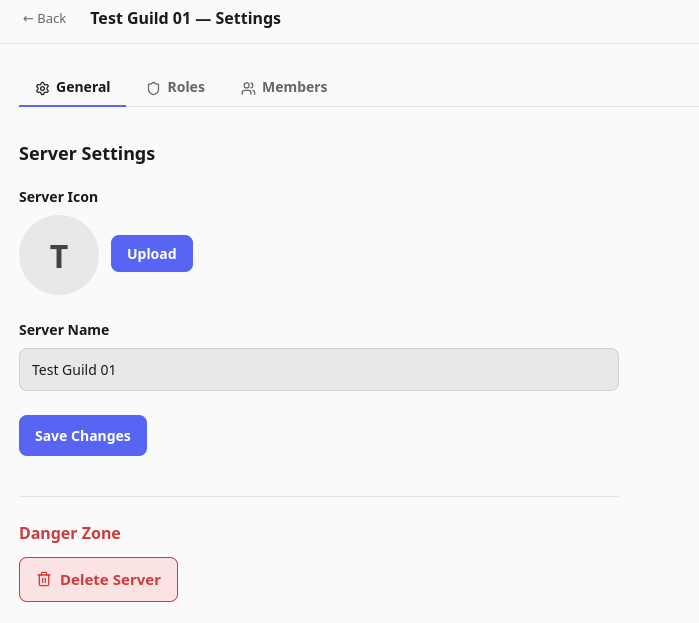
\includegraphics[width=0.5\textwidth]{guild_settings.png}
    \caption{Mockup: Server Settings Overview.}
    \label{fig:ui_guild_settings}
\end{figure}

\begin{figure}[H]
    \centering
    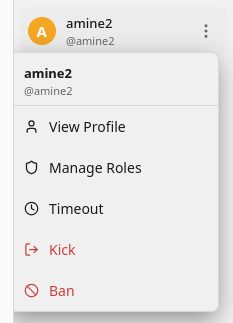
\includegraphics[width=0.3\textwidth]{guild_member_dropdown.png}
    \caption{Mockup: Member Action Menu.}
    \label{fig:ui_member_dropdown}
\end{figure}

\begin{figure}[H]
    \centering
    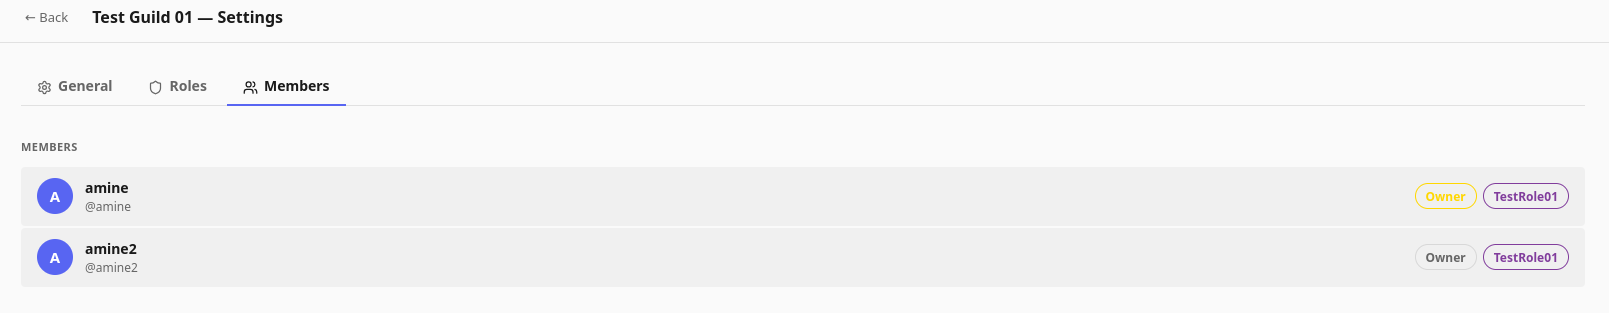
\includegraphics[width=0.5\textwidth]{guild_members_settings.png}
    \caption{Mockup: Member Management Interface.}
    \label{fig:ui_guild_members}
\end{figure}

\begin{figure}[H]
    \centering
    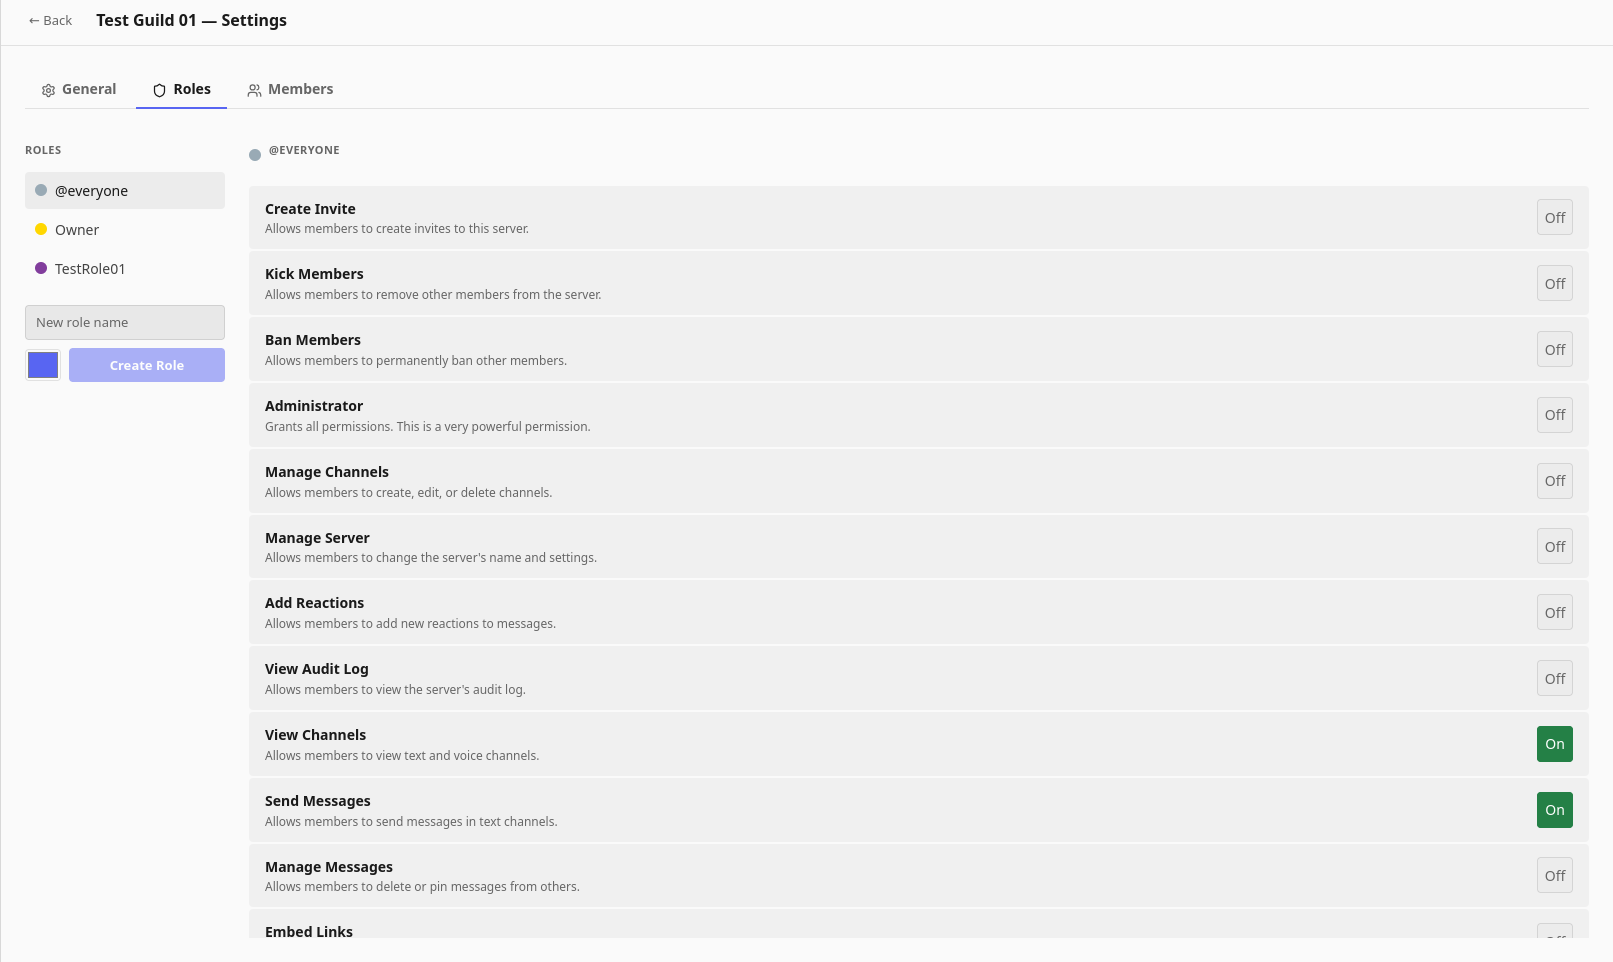
\includegraphics[width=0.5\textwidth]{guild_roles_settings.png}
    \caption{Mockup: Role Management Interface.}
    \label{fig:ui_guild_roles}
\end{figure}

\begin{figure}[H]
    \centering
    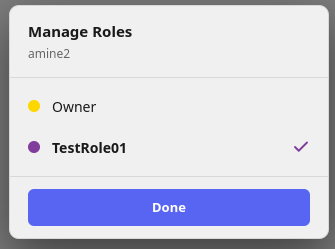
\includegraphics[width=0.4\textwidth]{member_manage_role.png}
    \caption{Mockup: Role Management and Member Administration.}
    \label{fig:ui_member_manage_role}
\end{figure}

\section{Conclusion}
This chapter presented Release 1 of our platform. By implementing secure authentication in Sprint 1 and server management with role-based access control in Sprint 2, we established the foundational infrastructure required for the encrypted messaging and P2P voice features detailed in Chapter 4.